\chapter{Processi e metodologie}
\label{chap:processi-metodologie}

\section{Contesto aziendale}

L'azienda si distingue per l'elevata attenzione rivolta all'organizzazione del lavoro e alla definizione dei processi di sviluppo, aspetti che hanno contribuito a creare un ambiente collaborativo ed efficiente. Grazie a una gestione strutturata delle attività, il team di sviluppo del progetto ErpAI ha potuto operare in maniera coordinata, favorendo una comunicazione efficace e una rapida risoluzione delle problematiche emerse durante lo sviluppo.

Il reparto dedicato al progetto ErpAI è composto da quattro sviluppatori, incluso il sottoscritto, coordinati dal titolare dell'azienda, che ha ricoperto un ruolo di supervisione, fornendo supporto tecnico e indicazioni progettuali durante l'intero periodo di sviluppo.

\subsection{Modello di sviluppo Agile}

L'azienda adotta il framework \textit{Scrum}\footnote{\cite{site:agile-manifesto}} come metodologia di sviluppo software, organizzando il lavoro in sprint della durata di una settimana.

Ogni sprint ha inizio con lo \textit{Sprint Planning}, incontro coordinato dallo \textit{Scrum Master}, figura responsabile del corretto svolgimento del processo Scrum. Durante questa fase vengono definite le funzionalità da sviluppare nel corso della settimana e vengono analizzate le criticità emerse durante la \textit{Sprint Retrospective} dello sprint precedente, con l'obiettivo di migliorare continuamente il processo di sviluppo.

Nel corso dello sprint, il team lavora in modo autonomo al raggiungimento degli obiettivi prefissati. Al termine della settimana si svolge la \textit{Sprint Review}, durante la quale vengono presentati i risultati ottenuti e raccolti i feedback necessari per valutare il lavoro svolto e pianificare le attività successive.

\begin{figure}[H]
\centering
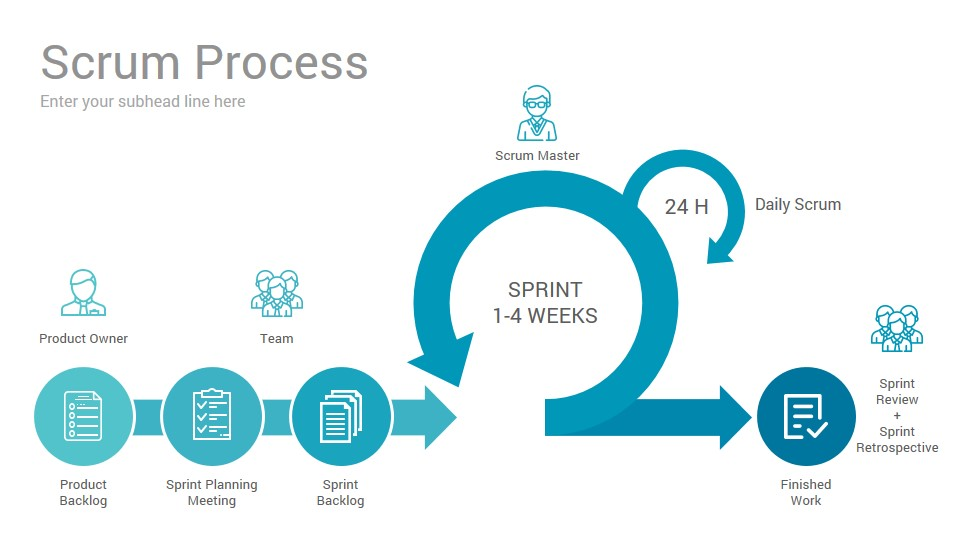
\includegraphics[alt={Modello Scrum}, height=5cm]{img/scrum.jpeg}
\caption{Modello Scrum}
\label{fig:scrum}
\end{figure}

\subsection{Issue Tracking System}

La gestione delle attività di sviluppo è affidata a Plane\footnote{\cite{site:plane}}, una piattaforma di \textit{issue tracking} che consente di organizzare e monitorare l'avanzamento del progetto attraverso una bacheca suddivisa nelle seguenti sezioni:

\begin{itemize}
\item \textbf{Backlog}: raccoglie le attività pianificate ma non ancora avviate;
\item \textbf{To Do}: contiene le attività pronte per essere sviluppate;
\item \textbf{In Progress}: comprende le attività attualmente in fase di sviluppo, revisione o testing;
\item \textbf{Done}: raccoglie le attività completate e chiuse.
\end{itemize}

Ogni issue contiene una serie di informazioni utili alla gestione del lavoro, tra cui:

\begin{itemize}
\item \textbf{Titolo}: breve descrizione dell'attività da svolgere;
\item \textbf{Descrizione}: dettagli relativi ai requisiti e agli obiettivi dell'attività;
\item \textbf{Assegnatari}: sviluppatori responsabili della realizzazione dell'issue;
\item \textbf{Stato}: indica la fase del ciclo di sviluppo in cui si trova l'attività.
\end{itemize}

\subsection{Version Control}

La gestione del codice sorgente è affidata al sistema di controllo di versione \gls{git}, utilizzato tramite Gitea\footnote{\cite{site:gitea}}, una piattaforma open-source per l'hosting di repository Git all'interno dell'infrastruttura aziendale.

L'organizzazione dei branch si ispira al modello GitFlow, opportunamente adattato alle esigenze del team di sviluppo. In particolare, vengono utilizzate le seguenti tipologie di branch:

\begin{itemize}
\item \textbf{main}: contiene la versione stabile del software destinata alla produzione;
\item \textbf{dev}: rappresenta il ramo principale di integrazione delle funzionalità in fase di sviluppo;
\item \textbf{feature/<numero-issue>}: utilizzato per lo sviluppo di nuove funzionalità, identificate tramite il codice univoco dell'issue corrispondente;
\item \textbf{fix}: dedicato alla correzione di bug o anomalie riscontrate durante lo sviluppo;
\item \textbf{release}: utilizzato per preparare una nuova versione del software prima del rilascio.
\end{itemize}


\begin{figure}[H]
    \centering
    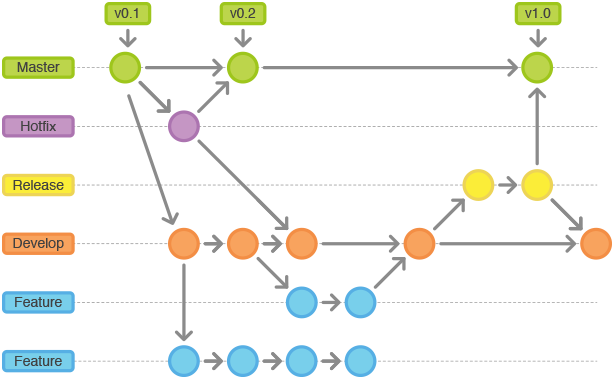
\includegraphics[alt={Modello GitFlow}, height=5cm]{img/gitflow.png}
    \caption{Modello GitFlow}
    \label{fig:gitflow}
\end{figure}
Prima dell'integrazione delle modifiche nei branch principali, il codice sviluppato viene sottoposto a un processo di \textit{code review} tramite \textit{pull request}. 
La creazione di una pull request è subordinata al superamento di alcuni controlli automatici di qualità del codice, tra cui l'analisi statica tramite PHPStan e le verifiche 
effettuate tramite Laravel Insight.\newline
La revisione da parte degli altri membri del team consente di individuare eventuali problematiche, verificare la conformità agli standard adottati e garantire una 
maggiore qualità del codice prima del suo inserimento nei rami condivisi del progetto.

\subsection{Il progetto}
Come anticipato nell'introduzione, il progetto di stage si inserisce nello sviluppo della quarta consegna di \textit{ErpAI}, un gestionale aziendale commissionato da Falmec S.p.A. 
Il sistema è progettato per supportare la pianificazione della produzione attraverso algoritmi di previsione delle vendite e il conseguente calcolo del mrp, 
consentendo di ottimizzare la gestione della produzione, del magazzino e dell'approvvigionamento dei materiali.

L'attività di stage si è concentrata sullo sviluppo di due componenti principali del sistema:

\begin{itemize}
    \item \textbf{Modulo XAI}: progettazione e integrazione di un chatbot auditabile all'interno del gestionale, in grado di fornire spiegazioni sulle decisioni prese dal sistema. 
    Il modulo consente inoltre di registrare tali spiegazioni e renderle successivamente consultabili tramite un sistema di storico (\textit{history}), garantendo tracciabilità 
    e auditabilità delle decisioni.
    \item \textbf{Sistema di alert}: progettazione e sviluppo di un motore di gestione degli alert finalizzato all'individuazione di criticità nei processi produttivi. 
    Il sistema permette inoltre agli utenti finali di definire e personalizzare regole di generazione degli alert in funzione delle specifiche esigenze operative.
\end{itemize}
Un ulteriore obiettivo dello stage consiste nell'integrare all'interno delle due componenti sviluppate alcune funzionalità introdotte nella terza consegna del progetto, in 
particolare un \textit{solver di scheduling}, responsabile della risoluzione di problemi di ottimizzazione relativi alla pianificazione delle attività e all'allocazione delle 
risorse disponibili. L'attività si limita tuttavia a integrazioni di carattere leggero, finalizzate a garantire la compatibilità tra il nuovo componente e le funzionalità 
sviluppate durante lo stage.

\subsection{Pianificazione delle attività}
Lo stage si è sviluppato nell'arco di 300 ore complessive, distribuite su sette settimane lavorative da 40 ore ciascuna e un'ultima settimana conclusiva da 20 ore.
\newline
Le prime due settimane sono state dedicate all'inserimento nel contesto progettuale, attraverso lo studio delle tecnologie adottate dall'azienda, necessarie per lo sviluppo 
delle componenti previste, l'analisi del lavoro precedentemente svolto dagli altri membri del team e la definizione dei requisiti funzionali che le componenti realizzate 
durante lo stage avrebbero dovuto soddisfare.
\newline
Le settimane successive sono state principalmente dedicate all'attività di sviluppo e integrazione delle funzionalità previste dal progetto. Le ultime 40 ore sono state 
invece destinate alle attività di testing, alla verifica del corretto funzionamento delle componenti implementate e alla produzione della documentazione tecnica relativa al 
lavoro svolto, con l'obiettivo di garantire la manutenibilità, l'estendibilità e l'auditabilità del codice prodotto.

\subsection{Modalità di lavoro e collaborazione}
L'attività di tirocinio è stata svolta interamente in presenza, favorendo un confronto diretto e continuo con il tutor aziendale e con gli altri sviluppatori coinvolti nel 
progetto \textit{ErpAI}.
\newline
Oltre agli incontri quotidiani dedicati all'allineamento sulle attività svolte e sulle problematiche emerse, il team ha utilizzato strumenti di comunicazione asincrona per 
la gestione di dubbi o criticità di minore entità. Questo ha permesso di ottenere rapidamente chiarimenti e feedback, mantenendo un flusso di collaborazione costante anche al 
di fuori degli incontri programmati.

\subsection{Analisi preventiva dei rischi}

Durante la fase iniziale dello stage sono stati identificati alcuni possibili rischi che avrebbero potuto influenzare il corretto svolgimento delle attività previste. Per ciascun rischio sono state individuate opportune strategie di mitigazione volte a ridurne l'impatto sul progetto.

\subsubsection{Integrazione con componenti esistenti}

\textbf{Descrizione:}
Il progetto prevede l'integrazione di nuove funzionalità, come il modulo XAI e il sistema di alert, all'interno di un gestionale già sviluppato. La conoscenza iniziale 
limitata dell'architettura esistente e delle logiche implementate avrebbe potuto causare difficoltà nell'individuazione dei punti corretti di integrazione.

\textbf{Soluzione:}
Prima dell'inizio dello sviluppo è stata prevista una fase di analisi del codice esistente e delle componenti già implementate, al fine di comprendere l'architettura del 
sistema e identificare le modalità di integrazione più appropriate.

\subsubsection{Apprendimento di nuove tecnologie}

\textbf{Descrizione:}
Lo sviluppo delle nuove componenti richiede l'utilizzo di tecnologie e strumenti non necessariamente già conosciuti, comportando il rischio di un rallentamento delle 
attività dovuto alla necessità di acquisire nuove competenze.

\textbf{Soluzione:}
Le prime settimane dello stage sono state dedicate allo studio delle tecnologie adottate dall'azienda e alla familiarizzazione con l'ambiente di sviluppo, permettendo 
di ridurre il rischio di ritardi nelle successive fasi di implementazione.

\subsubsection{Compatibilità con il solver di scheduling}

\textbf{Descrizione:}
L'integrazione con il solver di scheduling sviluppato nelle precedenti consegne potrebbe introdurre problematiche di compatibilità tra le componenti, dovute a differenze 
nelle interfacce o nelle modalità di gestione dei dati.

\textbf{Soluzione:}
L'integrazione è stata pianificata attraverso un'analisi preventiva delle interfacce esposte dal solver e una definizione delle modalità di comunicazione necessarie, 
limitando l'intervento alle modifiche strettamente necessarie.

\subsubsection{Tempi di risposta del sistema}

\textbf{Descrizione:}
L'integrazione di funzionalità basate su intelligenza artificiale, come il chatbot XAI, può introdurre un aumento dei tempi di risposta rispetto alle funzionalità 
tradizionali del gestionale. Tempi di elaborazione elevati potrebbero compromettere l'esperienza dell'utente e rendere meno efficace l'interazione con il sistema.

\textbf{Soluzione:}
È stata prevista un'analisi delle tempistiche di risposta delle componenti coinvolte, valutando eventuali ottimizzazioni nelle modalità di comunicazione e nella gestione 
delle richieste. Inoltre, sono state considerate strategie per migliorare la percezione dell'attesa da parte dell'utente, come la gestione asincrona delle operazioni più onerose.

\subsubsection{Integrazione con API e servizi esterni}

\textbf{Descrizione:}
Il funzionamento del modulo XAI richiede l'integrazione con API esterne per l'elaborazione delle richieste al modello linguistico. Tale dipendenza introduce possibili 
rischi legati alla disponibilità del servizio, alla gestione degli errori nelle comunicazioni e alla compatibilità tra le interfacce utilizzate.

\textbf{Soluzione:}
L'integrazione è stata progettata attraverso una separazione tra la logica applicativa del gestionale e i servizi esterni utilizzati, prevedendo una gestione controllata 
delle chiamate API e degli eventuali errori restituiti. Sono inoltre state effettuate verifiche preliminari sulle modalità di comunicazione e sui dati scambiati tra i diversi 
componenti.

\section{Obiettivi dello stage}

\begin{center}
    \rowcolors{2}{lightblue}{white}
        \begin{tabularx}{\textwidth}{|l|X|l|}
            \hline
            \rowcolor{gold}
            \textbf{Codice}  & \textbf{Descrizione requisito}  & \textbf{Tipologia}   \\
            \hline
            \textbf{O01} & Implementare un sistema XAI auditabile per registrare e consultare decisioni, fattori, evidenze e snapshot dei dati & Obbligatorio\\
            \hline
            \textbf{O02} & Realizzare regole alert, eventi e notifiche configurabili per segnalare proattivamente criticità operative. & Obbligatorio\\
            \hline
            \textbf{O03} & Integrare i punti decisionali della terza consegna nei log XAI e negli alert, limitandosi a controlli, riprese in mano e integrazioni leggere. & Obbligatorio\\
            \hline
            \textbf{D01} & Differenziare le spiegazioni XAI e i dettagli visibili in base al ruolo dell'utente. & Desiderabile\\
            \hline
            \textbf{D02} & Predisporre run di ottimizzazione tracciabili con input, output, score, metriche e log decisionale associato. & Desiderabile\\
            \hline
            \textbf{D03} & Introdurre dashboard o riepiloghi sugli alert generati, presi in carico e risolti. & Desiderabile\\
            \hline
            \textbf{F01} & Collegare un solver o microservizio esterno per scenari specialistici come nesting laser o sequenziamento avanzato. & Funzionale\\
            \hline
            \textbf{F02} & Aggiungere suggerimenti automatici di configurazione soglie basati sui dati storici. & Funzionale\\
            \hline
            \textbf{F03} & Integrare le spiegazioni XAI nel chatbot sviluppato da un altro piano di lavoro o modulo parallelo. & Funzionale\\
            \hline
        \end{tabularx}
\end{center}




\newpage